\documentclass[12pt,a4paper,titlepage,final]{report}
\usepackage{titlesec}
\usepackage{titlesec}
\titleformat{\chapter}{}{}{0em}{\bf\LARGE}

\usepackage{etoolbox}
\makeatletter
\patchcmd{\chapter}{\if@openright\cleardoublepage\else\clearpage\fi}{}{}{}
\makeatother

%%%%%%%%%%%%%%%%%%%%%%%%%%%%%%%%%%%%%%%%%
%\input{config.tex}
%%%%%%%%%%%%%%%%%%%%%%%%%%%%%%%%%%%%%%%%%
\usepackage{czech}
\usepackage[utf8]{inputenc}
\usepackage{times}


\usepackage[bookmarksopen,colorlinks,plainpages=false,urlcolor=blue]{hyperref}
\usepackage{url}

\usepackage{ifpdf}

% graphicx package for images
\usepackage{graphicx}
\usepackage{epstopdf}

\usepackage[top=2cm, left=2cm, text={17cm, 26cm}, ignorefoot]{geometry}
%%%%%%%%%%%%%%%%%%%%%%%%%%%%%%%%%

% landscape orientation for pages
\usepackage{pdflscape}
\usepackage{rotating}

% math symbols
\usepackage{amsmath}

% thick table borders
\usepackage{array}

\makeatletter
\newcommand{\thickhline}{%
    \noalign {\ifnum 0=`}\fi \hrule height 1pt
    \futurelet \reserved@a \@xhline
}
\newcolumntype{"}{@{\hskip\tabcolsep\vrule width 1pt\hskip\tabcolsep}}
\makeatother

% url packages
%\usepackage[bookmarksopen,colorlinks,plainpages=false,urlcolor=blue,unicode]{hyperref}
\usepackage{url}
\usepackage{xcolor}
\usepackage{hyperref}
%%%%%%%%%%%%%%%%%%%%%%%%%%%%%%%%%

\begin{document}

%%%%%%%%%%%%%%%%%%%%%%%%%%%%%%%%%%%%%%%%%%%%%%%%%%%%%%%%%%%%%%%%%%%%%%%%%%%%%%
% titulní strana
\def\projname{Dokumentace k projektu IFJ/IAL}
\def\projname{Implementace interpretu\\ imperativního jazyka IFJ14}
\begin{titlepage}
% \vspace*{1cm}
\begin{figure}[!h]
\centering

\includegraphics[height=6cm]{img/czlogo}
\end{figure}
\vfill
\begin{center}
\bigskip
\begin{large}
Dokumentace k projektu IFJ/IAL\\
\end{large}
\begin{Huge}
\projname\\
\end{Huge}
\end{center}
\vfill
\begin{center}
\begin{Large}
\today
\end{Large}
\end{center}
\vfill
\begin{flushleft}
\begin{large}
Tým 004, varianta a/2/II\\
\vfill
Norbert Ďurčanský - vedoucí (xdurca01), 20\% \\
Jindřich Dudek (xdudek04), 20\% \\
Jiří Dostál (xdosta40), 20\% \\
Ján Jusko (xjusko00), 20\% \\
Natalya Loginova (xlogin00), 20\% \\
\end{large}
\end{flushleft}
\end{titlepage}
%%%%%%%%%%%%%%%%%%%%%%%%%%%%%%%%%%%%%%%%%%%%%%%%%%%%%%%%%%%%%%%%%%%

\pagestyle{plain}
\pagenumbering{roman}
\setcounter{page}{1}
{\hypersetup{linkcolor=black}
\tableofcontents
}

\newpage
\pagestyle{plain}
\pagenumbering{arabic}
\setcounter{page}{1}


%%%%%%%%%%%%%%%%%%%%%%%%%%%%%%%%%%%%%%%%%%%%%%%%%%%%%%%%%%%%%%%%%%% 
\chapter{Úvod} \label{uvod}
Tato dokumentace obsahuje popis implementace interpretu imperativního jazyka IFJ14. Program načítá a interpretuje zdrojový soubor zapsaný v jazyce IFJ14. Jestliže interpret vyhodnotí kód jako spravný, pak se vrací návratová hodnota 0. V opačném případě program vrací kód chyby.

%%%%%%%%%%%%%%%%%%%%%%%%%%%%%%%%%%%%%%%%%%%%%%%%%%%%%%%%%%%%%%%%%%%
\chapter{Zadání} \label{zadani}
Jazyk IFJ14 je podmnožinou jazyka Pascal, což je staticky typovaný (tj. jednotlivé proměnné mají předem určen datový typ svou definicí) procedurální jazyk. Jazyk je case insensitive (nezáleží na velikosti písmen).

Interpret se skládá ze tří hlavních částí: (1) lexikální analyzátor (neboli scanner), (2) syntaktický analyzátor (parser), který je nejdůležitější částí programu, (3) interpret. Scanner načítá zdrojový soubor a rozpoznává ve zdrojovém kódu jednotlivé lexikální jednotky, parser pak zkontroluje sintaxi, provede sémantické akce a vygeneruje 3-adresný kód, který interpret vykoná.

Kromě toho interpret poskytuje některé vestavěné funkce včetně vyhledávání podřetězce v řetězci a řazení znaků v řetězci.

Náš tým řešil variantu zadání projektu a/2/II:
\begin{itemize}
\item Knuth-Morris-Prattův vyhledávací algoritmus
\item Řazení metodou Heap sort
\item Implementace tabulky symbolů pomocí hashovací tabulky
\end{itemize}

%%%%%%%%%%%%%%%%%%%%%%%%%%%%%%%%%%%%%%%%%%%%%%%%%%%%%%%%%%%%%%%%%%% 
\chapter{Implementace} \label{implementace}
V této kapitole je popsána implementace jednotlivých částí programu.

%=================================================================%
\section{Lexikální analyzátor}
Lexikální analyzátor (scanner) rozpoznává jednotlivé lexémy (lexikální jednotky) zdrojového programů a vytváří korespondující tokeny, přičemž komentáře a bílé znaky jsou vynechány (nikam se neukládají). Tokeny odpovídají lexikálním prvkům zdrojového kódu (například identifikátory, datové typy, klíčová slova, literály atd.) a kromě typu lexému obsahují důležité doplňující informace pro sémantickou analýzu a interpretaci (např. jméno identifikátoru, konkrétní hodnotu konstanty apod.).

Implementace lexikálního analyzátoru je založena na využití konečného automatu, který je realizován pomocí řídící konstrukce switch spolu s řídící proměnnou, která uchovává aktuální stav automatu. Scanner vrácí na požádání jeden token, který následuje za předešlým již načteným tokenem. Implementace je prováděna funkcí \texttt{getnextToken}, která přijímá ukazatel na strukturu reprezentující poslední načtený token a vrací celé číslo reprezentující buď kód chyby, v případě, že na chybu narazí, nebo typ aktuálního tokenu a současně strukturu jej reprezentující (prostřednictvím parametru) v případě úspěchu.

Diagram konečného automatu, který specifikuje lexikální analyzátor je příloze č. 1.

%=================================================================%
\section{Syntaktický analyzátor}
Syntaktický analýzátor (parser) je srdcem překladače. Jeho úkolem je zkontrolovat syntaxi vstupního programu, provést korespondující sémantické akce a vygenerovat tříadresný kód (tj. posloupnost tříadresných instrukcí), jež bude následně interpretován interpretem.

Parser načíta posloupnost tokenů ze zdrojového kódu na vstupu pomocí lexikálního analyzátoru. Syntaktická analýza jazykových konstrukcí (deklarace/definice proměnných a funkcí, řídící/přiřazovací příkazy apod.) je implementována pomocí rekurzivního sestupu podle pravidel LL gramatiky metodou shora dolů. Výrazy se zpracovávají pomocí precedenčního syntaktického analyzátoru, pracujícího zdola nahoru. Pak se pomocí funkce \texttt{generate\_inst} generuje instrukční list.

Pravidla LL gramatiky jsou v příloze č. 2, precedenční tabulka je v příloze č. 3.

%=================================================================%
\section{Interpret}
Základní funkce interpretu je vykonání vnitřního kódu vygenerovaného syntaktickým analyzátorem. Interpret tedy podle instrukcí zpracuje vstup programu a vygeneruje výstup.

Implementace je založena na tom, že interpret prochází instrukčním listem vnitřního kódu (který je implementován pomocí nekonečného pole) a postupně vykoná jednotlivé instrukce. Podpora instrukcí skoku je zajištěna použitím zásobníku a tabulek symbolů.

Samotná instrukce je reprezentována strukturou, která obsahuje operandy instrukce a některé další pomocné informace.

%=================================================================%
\section{Vyhledávání podřetězce v řetězci}
Podle varianty zadání vyhledávání podřetězce v řetězci je implementováno pomocí Knuth-Morris-Prattova vyhledávacího algoritmu (verze z přednášek IAL).

Knuth-Morris-Prattův algoritmus (KMP) využívá ke své práci konečný automat, který je reprezentován vzorkem P a vektorem FAIL, který má prvky typu integer, reprezentující cílový index zpětné šipky. Z každého uzlu automatu vychází dvě hrany - ANO (shoda znaku) a NE (neshoda). Automat načítá znaky, pokud dojde ke shodě, posune se na další stav, v případě neshody se vrátí na stav specifikovaný vektorem FAIL. Dosažení koncového stavu znamená nalezení vzorku.

Algoritmus má složitost O(n+m), kde n je délka prohledávaného textu, m je délka vyhledávaného vzorku.

%=================================================================%
\section{Řazení}
Podle varianty zadání řazení je implementováno pomocí algoritmu Heap Sort (verze z přednášek IAL).

Základní myšlenkou řadící metody Heap Sort je využítí hromady (heap) - struktury, založené na binárním stromu, u níž pro všechny uzly platí, že mezi otcovským uzlem a všemi jeho synovskými uzly je stejná relace uspořádání. Pomocí této struktury lze seřadit dodaná data prostě pomocí jejich vložení do hromady a následného postupného vybírání největšího/nejmenšího prvku. Podstatou řadicí metody je implementace hromady polem, která stanoví implicitní zřetězení prvků hromady.

Metoda Heap Sort má linearitmickou složitost O(N*log N), je nestabilní a není přirozená.

%=================================================================%
\section{Tabulka symbolů}
Tabulka symbolů v našem řešení byla realizována pomocí hashovací tabulky, která uchovává identifikátory funkcí, proměnných a další důležité informace s nimi spojené. K vyhledávání a vkládaní dat do tabulky je využita hashovací funkce, která generuje pozici uložení v hashovací tabulce na základě názvu identifikátoru, který tak zároveň slouží jako klíč pro vyhledávání. S tabulkou symbolů se pracuje pomocí funkcí uvozených názvem \texttt{hashtable\_} , které lze nalézt v modulu ial.c.

%%%%%%%%%%%%%%%%%%%%%%%%%%%%%%%%%%%%%%%%%%%%%%%%%%%%%%%%%%%%%%%%%%%
\chapter{Práce v týmu} \label{tym}
Ke komunikaci v týmu jsme využívali pravidelné schůze, kde jsme diskutovali řešení projektu, a vedoucí kontroloval stav plnění jednotlivých úkolů členy týmu. Kromě toho se používaly i jiné komunikační nástroje jako Skype a soukromá diskusní skupina.

Pro management zdrojového kódu jsme využívali systém správy verzí Git.

Rozdělení práce mezi členy týmu:\\
Norbert Ďurčanský (vedoucí) - vedoucí programátor, analýza a realizace algoritmů.\\
Jindřich Dudek - pomocný programátor.\\
Jiří Dostál - návrh, tvorba a aplikace testů.\\
Ján Jusko - pomocný programátor.\\
Natalya Loginova - vestavěné funkce, dokumentace. \\

%%%%%%%%%%%%%%%%%%%%%%%%%%%%%%%%%%%%%%%%%%%%%%%%%%%%%%%%%%%%%%%%%%%
\chapter{Literatura} \label{literatura}
\begin{enumerate}
  \item CORMEN, Thomas H. Introduction to algorithms. 3rd ed. Cambridge: MIT Press, 2009. ISBN 978-0-262-03384-8.
  \item MEDUNA, Alexander. Formal languages and computation: models and their applications. Boca Raton: CRC Press, 2014. ISBN 978-1-4665-1345-7.
\end{enumerate}
\newpage
%%%%%%%%%%%%%%%%%%%%%%%%%%%%%%%%%%%%%%%%%%%%%%%%%%%%%%%%%%%%%%%%%%% 
\appendix
\clearpage% Flush earlier floats (otherwise order might not be correct)
\thispagestyle{empty}% empty page style 
\chapter{Přílohy} \label{prilohy}
%=================================================================%
\section{Pravidla LL gramatiky}
1. \textless PROGRAM\textgreater  $\rightarrow$ var \textless DECLARELIST\textgreater  begin \textless PROG\textgreater \\
2. \textless PROGRAM\textgreater  $\rightarrow$ begin \textless PROG\textgreater \\
3. \textless PROGRAM\textgreater  $\rightarrow$ function \textless FUNCTION\textgreater  forward; \\
4. \textless PROGRAM\textgreater  $\rightarrow$ function \textless FUNCTION\textgreater ; \textless PROGFUNCTION\textgreater \\
5. \textless FUNCTION\textgreater  $\rightarrow$ id(\textless FUN\_PARAMS\textgreater ); \\
6. \textless FUN\_PARAMS\textgreater  $\rightarrow$ id:\textless DTYPE\textgreater ; \textless FUN\_PARAMS\textgreater \\
7. \textless FUN\_PARAMS\textgreater  $\rightarrow$ $\varepsilon$ \\
8. \textless DTYPE\textgreater  $\rightarrow$ integer \\
9. \textless DTYPE\textgreater  $\rightarrow$ real \\
10. \textless DTYPE\textgreater  $\rightarrow$ string \\
11. \textless DTYPE\textgreater  $\rightarrow$ boolean \\
12. \textless PROGFUNCTION\textgreater  $\rightarrow$ begin \textless PROGCONDITION\textgreater \\
13. \textless PROGFUNCTION\textgreater  $\rightarrow$ id \textless COMMAND\textgreater \\
14. \textless PROGFUNCTION\textgreater  $\rightarrow$ while \textless COMMAND\textgreater \\
15. \textless PROGFUNCTION\textgreater  $\rightarrow$ if \textless COMMAND\textgreater \\
16. \textless PROGFUNCTION\textgreater  $\rightarrow$ write \textless COMMAND\textgreater \\
17. \textless PROGFUNCTION\textgreater  $\rightarrow$ readln \textless COMMAND\textgreater \\
18. \textless COMMAND\textgreater  $\rightarrow$ id:= \\
19. \textless COMMAND\textgreater  $\rightarrow$ readln(id) \\
20. \textless COMMAND\textgreater  $\rightarrow$ write(\textless TERM\textgreater ) \\
21. \textless TERM\textgreater  $\rightarrow$ id \\
22. \textless TERM\textgreater  $\rightarrow$ const\_string \\
23. \textless TERM\textgreater  $\rightarrow$ const \\
24. \textless COMMAND\textgreater  $\rightarrow$ while \textless PRECEDENCE\textgreater  do begin \textless PROGCONDITION\textgreater \\
25. \textless COMMAND\textgreater  $\rightarrow$ if \textless PRECEDENCE\textgreater  then begin \textless PROGCONDITION\textgreater \\
26. \textless PROGCONDITION\textgreater  $\rightarrow$ \textless COMMAND\textgreater  else begin \textless PROGFUNCTION\textgreater \\
27. \textless LIBRARYFUNCTION\textgreater  $\rightarrow$ length(id) \\
28. \textless LIBRARYFUNCTION\textgreater  $\rightarrow$ length(const\_string) \\
29. \textless LIBRARYFUNCTION\textgreater  $\rightarrow$ copy(id,id,id) \\
30. \textless LIBRARYFUNCTION\textgreater  $\rightarrow$ copy(id,const,id) \\
31. \textless LIBRARYFUNCTION\textgreater  $\rightarrow$ copy(id,id,const) \\
32. \textless LIBRARYFUNCTION\textgreater  $\rightarrow$ copy(id,const,const) \\
33. \textless LIBRARYFUNCTION\textgreater  $\rightarrow$ copy(conststr,id,id) \\
34. \textless LIBRARYFUNCTION\textgreater  $\rightarrow$ copy(conststr,id,const) \\
35. \textless LIBRARYFUNCTION\textgreater  $\rightarrow$ copy(conststr,const,id) \\
36. \textless LIBRARYFUNCTION\textgreater  $\rightarrow$ copy(conststr,const,const) \\
37. \textless LIBRARYFUNCTION\textgreater  $\rightarrow$ find(id,id) \\
38. \textless LIBRARYFUNCTION\textgreater  $\rightarrow$ find(id,conststr) \\
39. \textless LIBRARYFUNCTION\textgreater  $\rightarrow$ find(conststr,id) \\
40. \textless LIBRARYFUNCTION\textgreater  $\rightarrow$ find(conststr,conststr) \\
41. \textless LIBRARYFUNCTION\textgreater  $\rightarrow$ sort(id) \\
42. \textless LIBRARYFUNCTION\textgreater  $\rightarrow$ sort(conststr) \\
\newpage
%=================================================================%
\begin{landscape}
\section{Konečný automat}
% \vspace*{1cm}
\begin{figure}[!h]
%\begin{sideways}
\centering
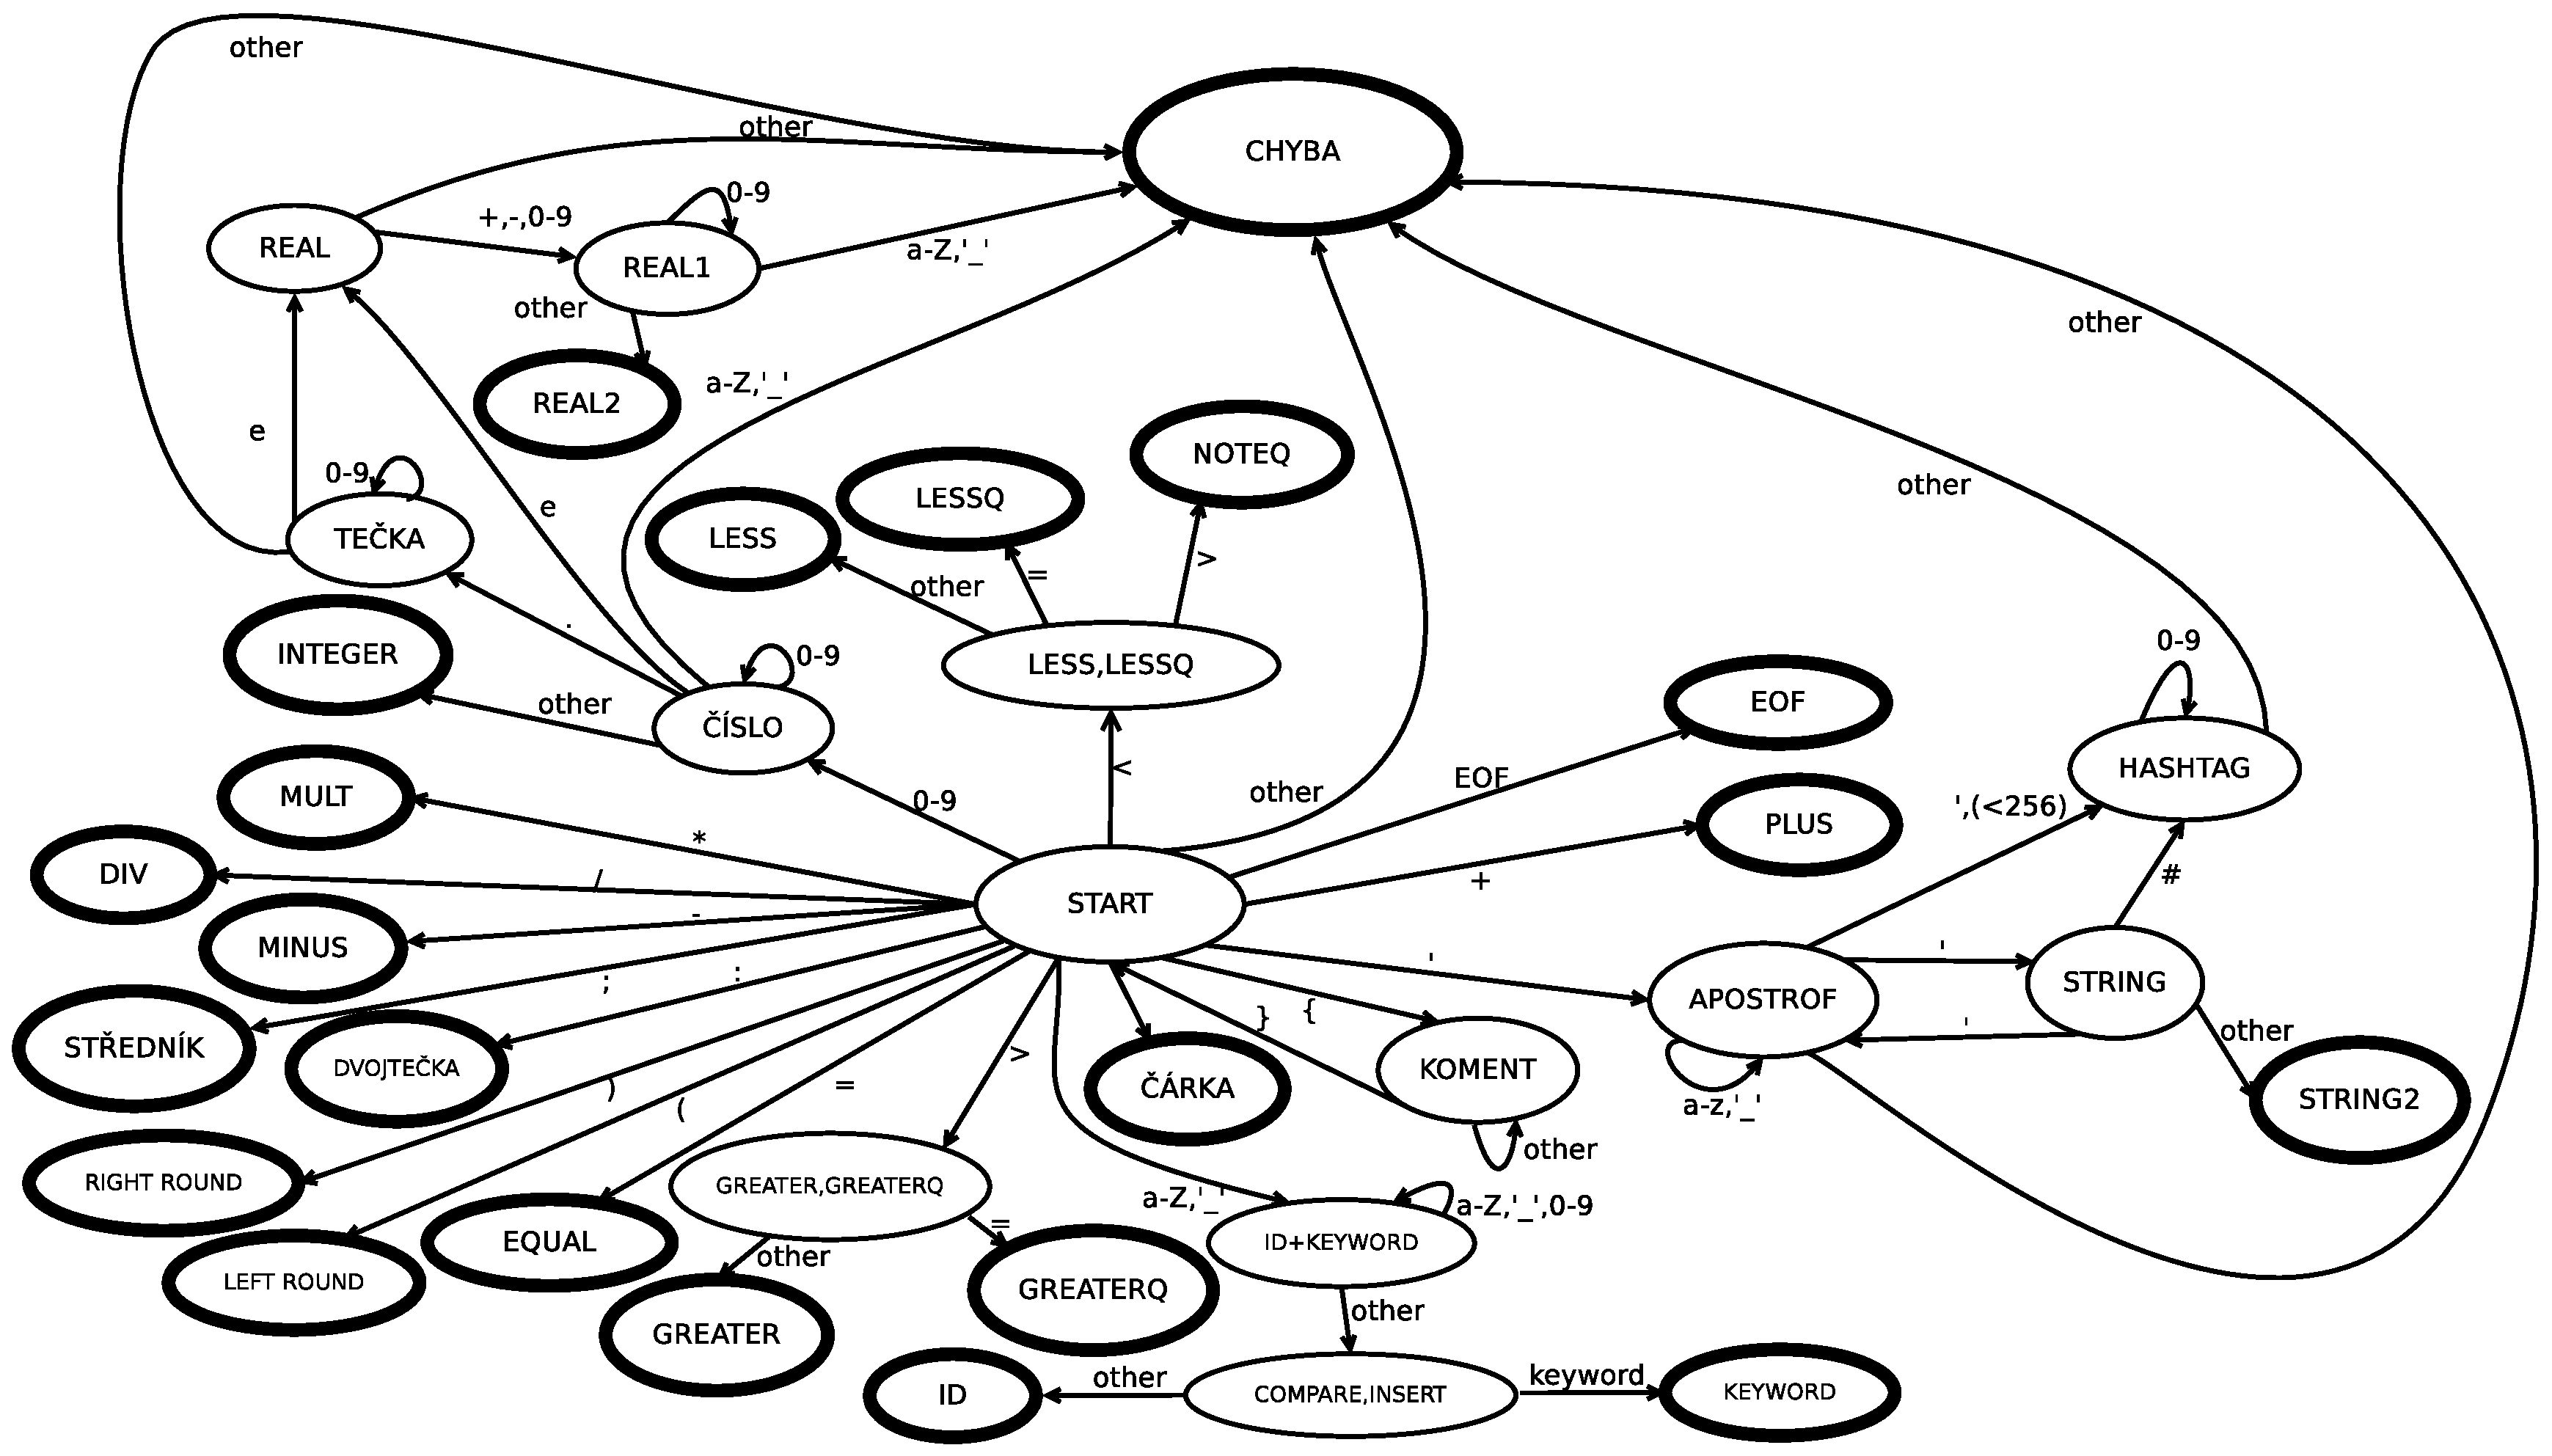
\includegraphics[height=350px]{img/IFJ_KA}
%\end{sideways}
\end{figure}
\end{landscape}
\clearpage% Flush page
\newpage
%\end{landscape}
%=================================================================%
%\clearpage% Flush earlier floats (otherwise order might not be correct)
%\thispagestyle{empty}% empty page style 
\begin{landscape}% Landscape page
\section{Precedenční tabulka}
\begin{table}[h]
\centering
\resizebox{\textwidth}{!}{%
\begin{tabular}{|c"c|c|c|c|c|c|c|c|c|c|c|c|c|}
\thickhline
                               & +   & -   & *   & /   & ID & ( & )   & \textless & \textgreater & $\geq$ & $\leq$ & \$   & \textless\textgreater \\ \thickhline
+                     & \textgreater & \textgreater & \textless    & \textless    & \textless   & \textless  & \textgreater & \textgreater       & \textgreater          & \textgreater  & \textgreater  & \textgreater & \textgreater                   \\ \hline
-                     & \textgreater & \textgreater & \textless    & \textless    & \textless   & \textless  & \textgreater & \textgreater       & \textgreater          & \textgreater  & \textgreater  & \textgreater & \textgreater                   \\ \hline
*                     & \textgreater & \textgreater & \textgreater & \textgreater & \textless   & \textless  & \textgreater & \textgreater       & \textgreater          & \textgreater  & \textgreater  & \textgreater & \textgreater                   \\ \hline
/                     & \textgreater & \textgreater & \textgreater & \textgreater & \textless   & \textless  & \textgreater & \textgreater       & \textgreater          & \textgreater  & \textgreater  & \textgreater & \textgreater                   \\ \hline
ID                    & \textgreater & \textgreater & \textgreater & \textgreater &             &            & \textgreater & \textgreater       & \textgreater          & \textgreater  & \textgreater  & \textgreater & \textgreater                   \\ \hline
(                     & \textless    & \textless    & \textless    & \textless    & \textless   & \textless  & =            & \textless          & \textless             & \textless     & \textless     &              & \textless                      \\ \hline
)                     & \textgreater & \textgreater & \textgreater & \textgreater &             &            & \textgreater & \textgreater       & \textgreater          & \textgreater  & \textgreater  & \textgreater & \textgreater                   \\ \hline
\textless             & \textless    & \textless    & \textless    & \textless    & \textless   & \textless  & \textgreater &                    &                       &               &               & \textgreater &                                \\ \hline
\textgreater          & \textless    & \textless    & \textless    & \textless    & \textless   & \textless  & \textgreater &                    &                       &               &               & \textgreater &                                \\ \hline
$\geq$                  & \textless    & \textless    & \textless    & \textless    & \textless   & \textless  & \textgreater &                    &                       &               &               & \textgreater &                                \\ \hline
$\leq$                  & \textless    & \textless    & \textless    & \textless    & \textless   & \textless  & \textgreater &                    &                       &               &               & \textgreater &                                \\ \hline
\$                     & \textless    & \textless    & \textless    & \textless    & \textless   & \textless  & \textless    & \textless          & \textless             & \textless     & \textless     & OK           & \textless                      \\ \hline
\textless\textgreater & \textless    & \textless    & \textless    & \textless    & \textless   & \textless  & \textgreater &                    &                       &               &               & \textgreater &                                \\ \thickhline
\end{tabular}
}
\end{table}

\end{landscape}
%\clearpage% Flush page
\newpage
%=================================================================%
\section{Metriky kódu}
\paragraph{Počet souborů:}  20 souborů
\paragraph{Počet řádků zdrojového textu:} 6564 řádků
\paragraph{Velikost spustitelného souboru:} 124.1 kB  (systém Linux, 32 bitová architektura, při překladu bez ladicích informací)


% % % % % % % % % % % % % % % % % % % % % % % % % % % % % % % % % % 

\end{document}